\renewcommand{\chaptername}{Cap\'itulo}
\chapter{Marco Te\'orico} 
\label{MarcoTeorico}

El cap\'titulo \ref{MarcoTeorico} se organiza como sigue: en primer lugar trata la importancia de los metadatos, considerados como datos descriptivos para los documentos de los repositorios. Posteriormente, se presenta el modelo de datos RDF y su contexto en la web sem\'antica, seguido de una breve descripci\'on del lenguaje de consulta est\'andar para datos en RDF, SPARQL. En la tesis, el acceso a los datos se implementa en servicios REST, por lo que se describen sus caracter\'isticas principales junto con los requerimientos para repositorios de acuerdo con la  \emph{Confederation of Open Access Repositories},  Confederaci\'on de Repositorios de Acceso Abierto (COAR). Finalmente, el cap\'titulo describe los trabajos relacionados. 

\section{La importancia de los metadatos}

Actualmente, en la web existe gran cantidad de informaci\'on sobre cualquier tema, tanta que se requiere del desarrollo de servicios que consideren su pertinencia, veracidad y  calidad para satisfacer necesidades de informaci\'on espec\'ificas de los usuarios tomando en cuenta aspectos t\'ecnicos de accesibilidad y disponibilidad, esto porque el acceso se realiza desde cualquier lugar y mediante una gama amplia de dispositivos.\newline

El etiquetado y descripci\'on de los contenidos son cruciales en el desarrollo de ese tipo de servicios, el primero permite categorizar o clasificar, el segundo se refiere al uso de las descripciones, elementos descriptores o \emph{metadatos} para que los recursos digitales se localicen y procesen adecuadamente por agentes tales como computadoras, aplicaciones m\'oviles y usarios con roles y caracter\'isticas propias. \newline

Seg\'un \cite{W3C}, una prio\-ri\-dad particular del \emph{World Wide Web Consortium}, (Consorcio W3C), es usar la web para documentar el significado de los metadatos. La importancia de la gesti\'on, uso y representaci\'on de los metadatos en modelos sem\'anticos u ontolog\'ias, se relaciona directamente con el modelo de datos conocido como Marco de Descripci\'on de Recursos, en ingl\'es \emph{Resource Description Framework}, (RDF). La secci\'on \ref{RDF} describe caracter\'isticas de este modelo junto con otras tecnolog\'ias de la web sem\'antica.\newline

\section{RDF en el contexto de la web sem\'antica}
\label{RDF}

La web es una plataforma tecnol\'ogica que constituye la mayor base de datos existente, se conforma por todo tipo de recursos, donde las personas o usuarios realizan tareas como publicar, explorar, consultar, almacenar datos e informaci\'on. En sus inicios, en la web se consideraba que los recursos debieran ser entendidos s\'olo por los usuarios, con el paso del tiempo y la gran cantidad de datos que est\'an en ella, es de suma importancia su gesti\'on y procesamiento mediado por las computadoras. \newline

La web sem\'antica, extensi\'on de la web tradicional, promueve el modelado, etiquetado y representaci\'on de la informaci\'on de manera que tanto los humanos como las computadoras sean capaces de ``comprender'' el contenido y la descripci\'on de los recursos; como menciona \cite{IntroBDRDF}, esta web propone una alternativa para agregar significado a los contenidos almacenados con el prop\'osito de propiciar una interacci\'on m\'as fluida entre aplicaciones, servicios, computadoras y el ser humano en comparaci\'on con la web tradicional. \newline

Las tecnolog\'ias de la web sem\'antica se rigen bajo ciertas normas y lenguajes est\'andar organizados en capas o niveles, como muestra la figura \ref{ModeloWebSemantica}, los cuales se describen a continuaci\'on \cite{IntroBDRDF}:

\begin{figure}[!ht]
    \centering
    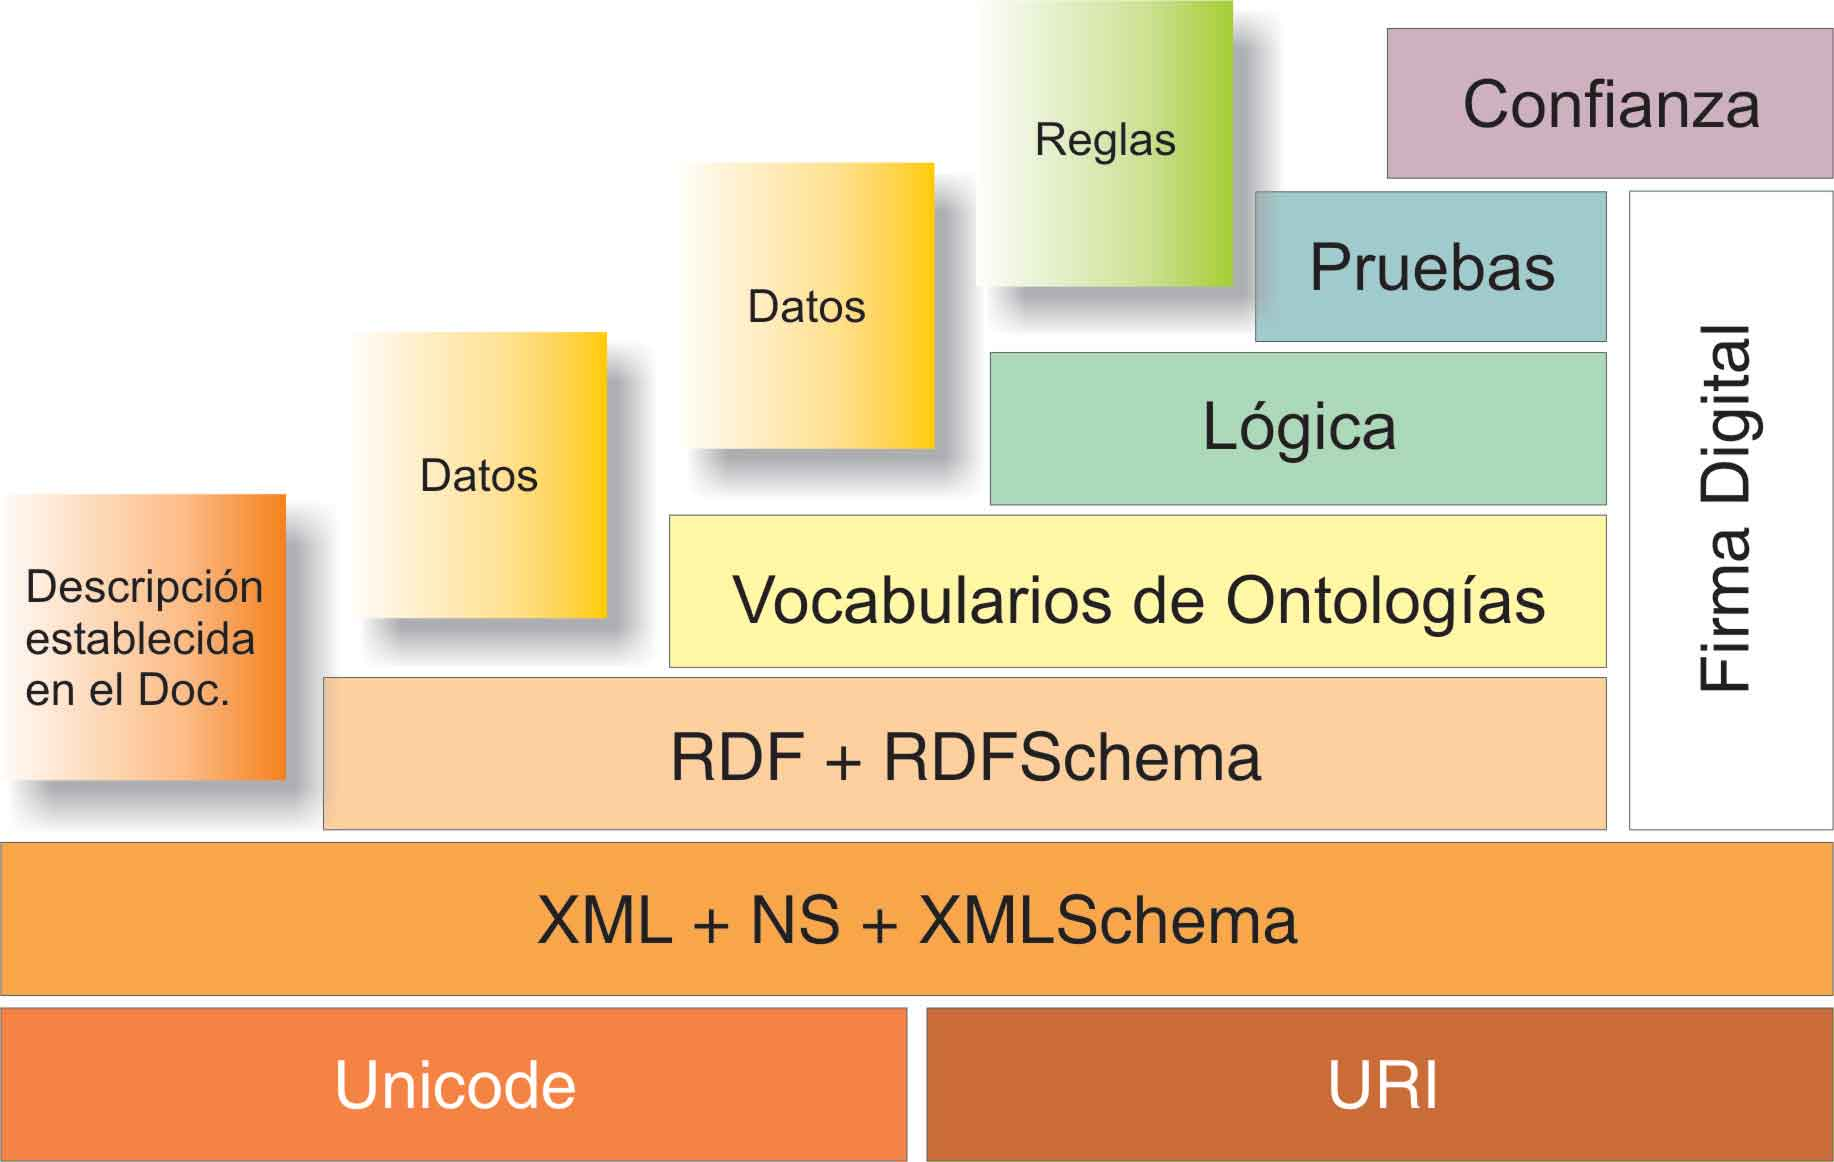
\includegraphics[width=10cm]{figures/ModeloCapasWebSemantica.jpg} %NOMBRE DE LA FIGURA y TAMAÑO
    \caption{Modelo de capas de Berners-Lee para la web sem\'antica\cite{WebSemanticaSciELO}} %PIE DE LA IMAGEN
    \label{ModeloWebSemantica}
\end{figure}

\begin{itemize}
    \item \textit{Unicode} \cite{W3C}. Est\'andar para documentos de texto que permite codificar la mayor\'ia de los sistemas de escritura del mundo.
    
    \item \textit{Uniform Resource Identifier}, (URI), identificador uniforme de recursos \cite{W3C}. Es\-t\'an\-dar para crear identificadores de recursos web a trav\'es de cadenas compactas de ca\-rac\-te\-res, identifican a los recursos de forma un\'ivoca, se emplean para localizarlos de forma autom\'atica. Un \textit{Uniform Resource Locator}, (URL), identificador de recursos uniforme, es un tipo de URI, por ejemplo, \texttt{http://informatica.uppuebla.edu.mx/} identifica espec\'ificamente a la p\'agina inicial de un servidor. 

    \item \textit{XML\footnote{\textit{eXtensible Markup language} (Lenguaje de Marcado Extensible o Lenguaje de Marcas Extensible)}} \cite{W3C}. Es un lenguaje de marcado similar a HTML, es una especificaci\'on del W3C de prop\'osito general en la que cada usuario define sus propias etiquetas. 
    
    \item \textit{XML namespaces} \cite{W3C}. Los espacios de nombre de XML se emplean para atender el problema de ambig\"{u}edad en los documentos XML de la web, de manera que cada elemento est\'a identificado por una URI que lo hace \'unico y universal. Los espacios de nombre son recomendaci\'on de W3C.
    
    \item RDF \cite{W3CSemanticWeb}. Modelo est\'andar para el intercambio de datos en la web, con caracter\'isticas que facilitan la fusi\'on de datos incluso en diferentes esquemas. RDF ampl\'ia la estructura de enlaces web (\emph{links}) para nombrar a dos recursos denominados \emph{sujeto} y \emph{objeto}, as\'i como a la relaci\'on entre ellos. Estos enunciados se conocen como \textit{ternas} o \emph{tripletas}. En el modelo de datos RDF se representan datos estructurados y semiestructurados o combinaciones, estos datos se comparten y utilizan por diferentes aplicaciones.
    
    \item \textit{RDF Schema} \cite{W3CRDFSchema}. Proporciona un vocabulario para el modelo de datos RDF, lo complementa con diferentes documentos anexos que describen los conceptos b\'asicos y la sintaxis abstracta de RDF. RDF Schema es una extensi\'on sem\'antica de RDF que proporciona mecanismos para describir grupos de recursos y sus relaciones, est\'a escrito en RDF, los recursos se utilizan para determinar las caracter\'isticas de otros recursos como dominio y rango de propiedades.
    
    
    \item \textit{Ontolog\'ia}. Seg\'un \cite{Ontologias}, una ontolog\'ia es un marco com\'un o una estructura conceptual sistematizada y de consenso no s\'olo para almacenar la informaci\'on, sino tambi\'en para poder buscarla y recuperarla. Una ontolog\'ia define los t\'erminos y las relaciones b\'asicas para la compresi\'on de un \'area del conocimiento o dominio, as\'i como las reglas para combinar los t\'erminos que definen las extensiones de este vocabulario controlado
    
    \item \textit{Vocabularios de ontolog\'ias}. El lenguaje de ontolog\'ias web, (\textit{Ontologies Web Language}), est\'a dise\~{n}ado para ser usado en aplicaciones que necesitan procesar el contenido de la informaci\'on,  cuenta con un vocabulario m\'as extenso al de RDF y RDF Schema, junto con una sem\'antica formal. OWL tiene tres sublenguajes que var\'ian por su nivel de expresividad: OWL Lite, OWL DL y OWL Full \cite{LaWebSemantica}
    
    \item \textit{Capa l\'ogica}. Permite determinar si la estructura de los razonamientos es v\'alida a trav\'es del estudio de las reglas formales. En esta capa se infiere conocimiento, requiere de la interacci\'on entre las ontolog\'ias y agentes de software, (programas o aplicaciones) \cite{LaWebSemantica}
    
    \item \textit{Capa de pruebas}. A trav\'es de demostraciones matem\'aticas se comprueba que el procesamiento del agente de software alcance la m\'axima confiabilidad en sus razonamientos \cite{LaWebSemantica}
    
    \item \textit{Capa de confianza}. Establece las pol\'iticas de seguridad que permitan asignar niveles de fiabilidad a determinados recursos, de forma comprobable por agentes. Esta capa usa firmas digitales y redes de confianza \cite{LaWebSemantica}

\end{itemize}

Los lenguajes utilizados ampliamente para representar los datos en la web sem\'antica son XML, RDF y OWL. El lenguaje de consulta para datos en RDF se describe en la secci\'on \ref{SPARQL}.

\section{SPARQL: lenguaje de consulta para datos en RDF}
\label{SPARQL}

RDF es un modelo de datos que se asocia con diferentes representaciones, una de ellas es como un modelo de grafos dirigidos etiquetados que representan informaci\'on en la web. Se emplea para representar informaci\'on personal, datos de redes sociales, metadatos sobre objetos digitales o como medio para la integraci\'on de fuentes de informaci\'on heterog\'eneas.\newline

Los datos en RDF se recuperan utilizando SPARQL, \textit{SPARQL protocol and RDF query language}, protocolo y lenguaje de consulta para RDF, sirve para extraer la informaci\'on contenida en una ontolog\'ia RDF, devuelve resultados en forma de enlaces o esquemas RDF. Entre sus especificaciones, de acuerdo con \cite{SkosSparql}, se encuentran las siguientes:

\begin{itemize}
    \item La especificaci\'on del protocolo SPARQL para RDF \textit{SPROT} que define el protocolo remoto para enviar consultas SPARQL y recibir los resultados
    \item La especificaci\'on del formato XML de los resultados de consultas SPARQL \textit{RESULTS}, define un formato de documento XML para representar los resultados de las consultas \texttt{SELECT} y \texttt{ASK} 
\end{itemize}

La Figura \ref{ejemploRDFgrafico} muestra una representaci\'on gr\'afica simple de \textit{vc-db-1.rdf}, archivo que contiene RDF para varias descripciones de vCard de personas, descritas en las notas del W3C ``Representaci\'on de objetos vCard en RDF / XML''.\newline

\begin{figure}[!ht]
    \centering
    \fbox{
    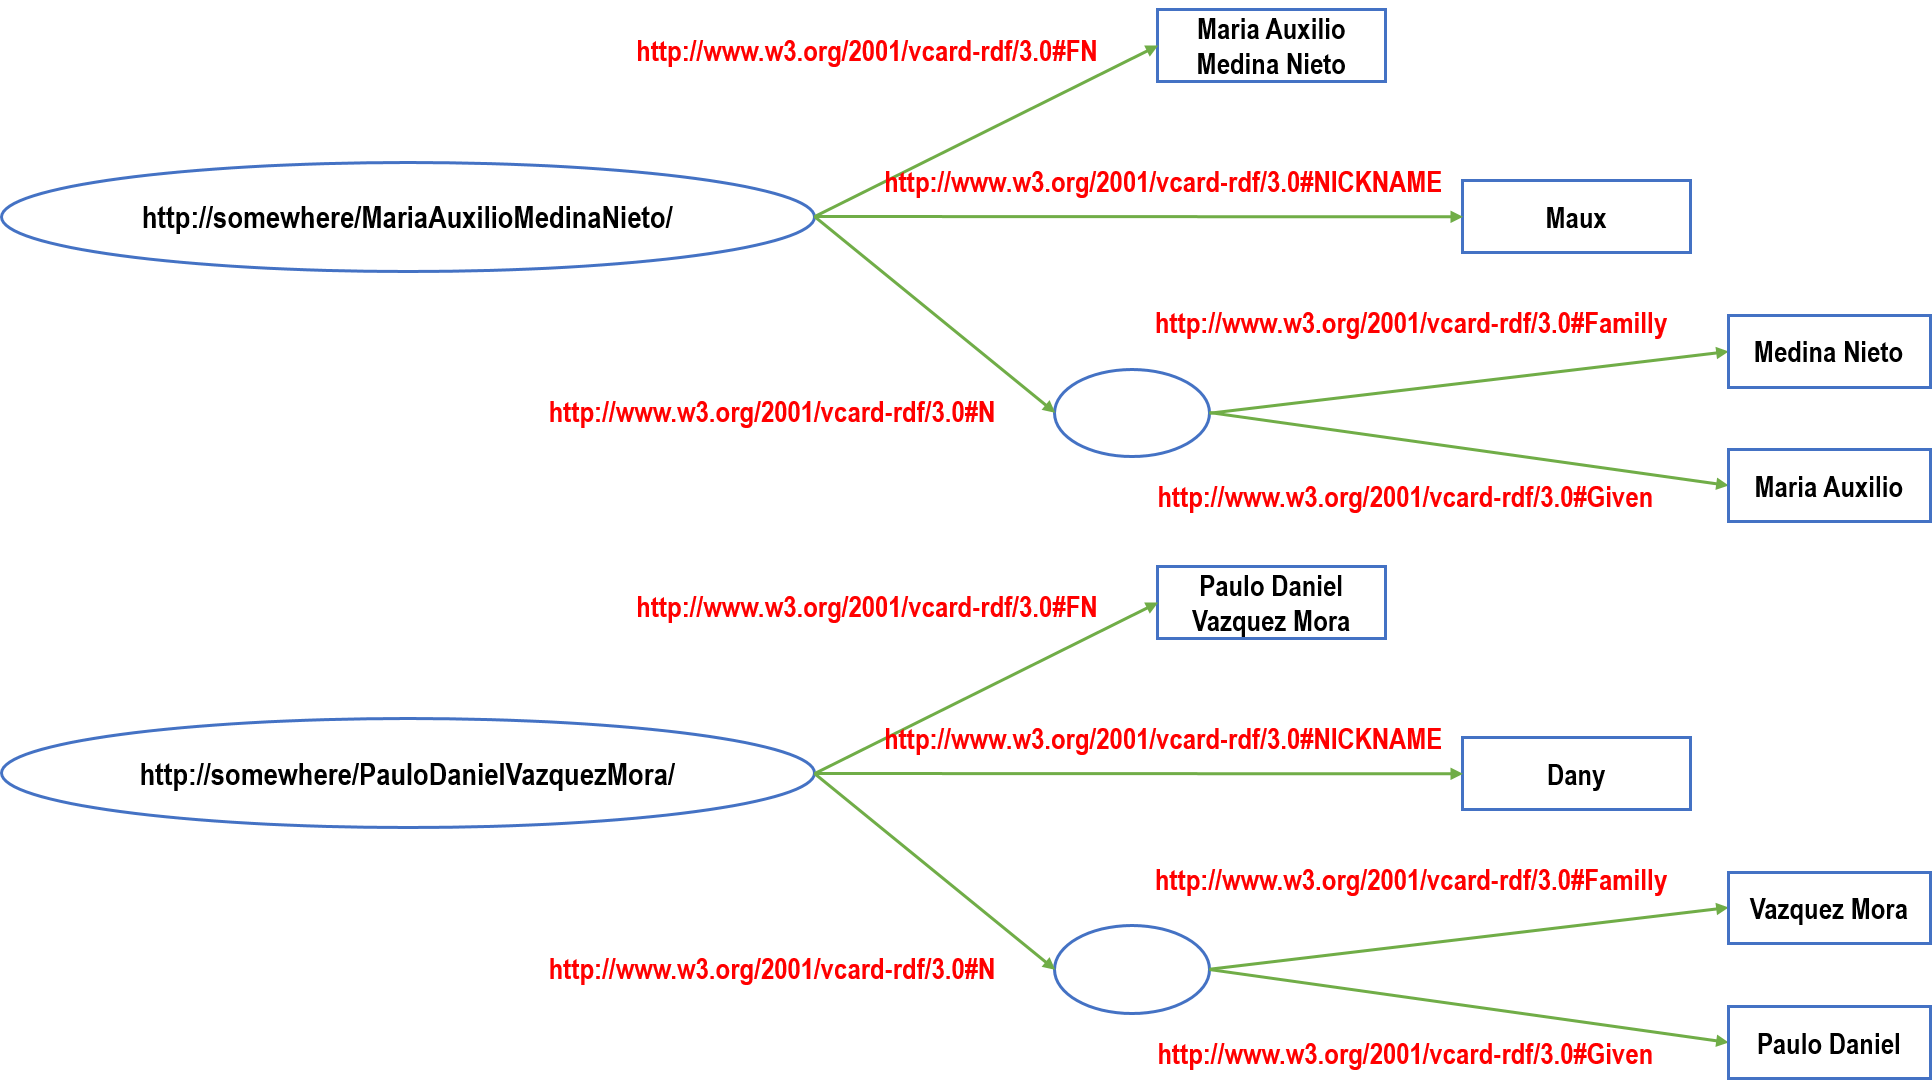
\includegraphics[scale=.44]{figures/vcdb.png}} 
    \caption{Ejemplo de representaci\'on gr\'afica provenientes de objetos vCard en RDF / XML} 
    \label{ejemploRDFgrafico}
\end{figure}

La Figura \ref{ejemploRDF} muestra el esquema RDF expresado como un conjunto de ternas, (tambi\'en llamadas tripletas).\newline

\begin{figure}[!ht]
    \centering
    \fbox{
    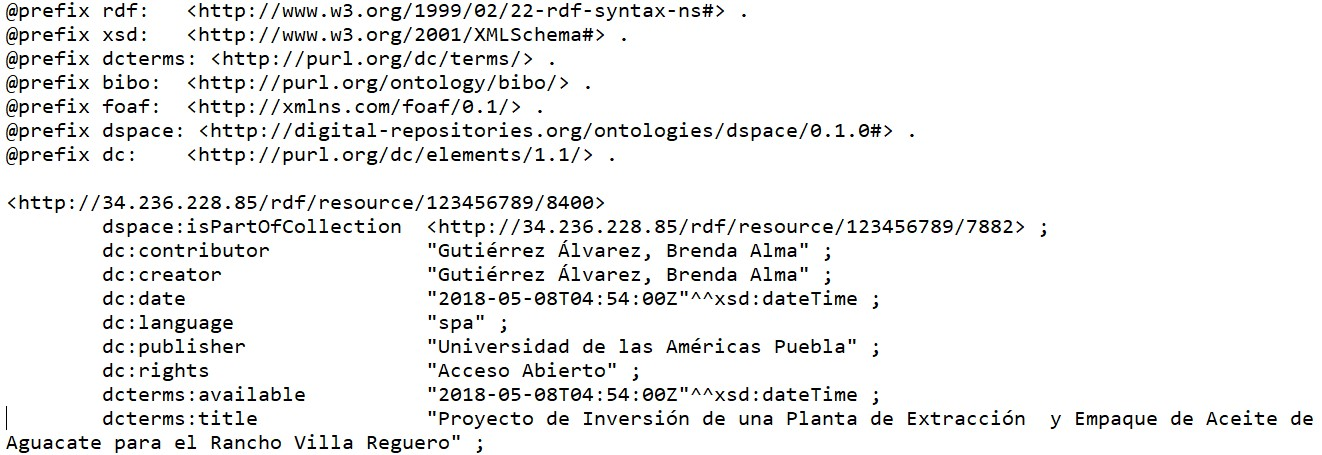
\includegraphics[scale=.45]{figures/ejemploRDF.jpg}} %NOMBRE DE LA FIGURA y TAMAÑO
    \caption{Ejemplo de conjunto de ternas en RDF} %PIE DE LA IMAGEN
    \label{ejemploRDF}
\end{figure}

    
\section{Servicios REST}

Los servicios REST se emplean para explotar recursos a partir de la migraci\'on a la web 2.0, sustituyen aquellos que hac\'ian uso de los protocolos SOAP y WSDL, su arquitectura es sencilla y est\'a orientada a recursos, hacen uso del protocolo HTTP. Los servicios \textit{Re\-pre\-sen\-ta\-tio\-nal State Transfer}, Transferencia de Estado Representacional (REST) cumplen con las premisas siguientes \cite{FeaturesREST}:

\begin{itemize}
    \item Se define una \emph{interfaz} de comunicaci\'on \emph{cliente-servidor} que separa las res\-pon\-sa\-bi\-li\-da\-des entre ambas partes como muestra la figura \ref{arquitecturaREST1}.
    
        \begin{figure}[!ht]
        \centering
        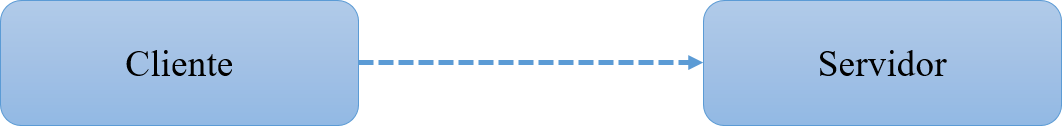
\includegraphics[width=10cm]{figures/ClienteServidorREST.png} 
        \caption{Arquitectura cliente servidor de servicio REST} 
        \label{arquitecturaREST1}
    \end{figure}

 \item Servicio web \emph{sin estado} ya que  cada petici\'on que se realiza es completamente independiente de cualquier otra, sin embargo, todas las solicitudes al mismo servicio son id\'enticas,  ver la Figura \ref{arquitecturaREST2}.
    
    \begin{figure}[!ht]
        \centering
        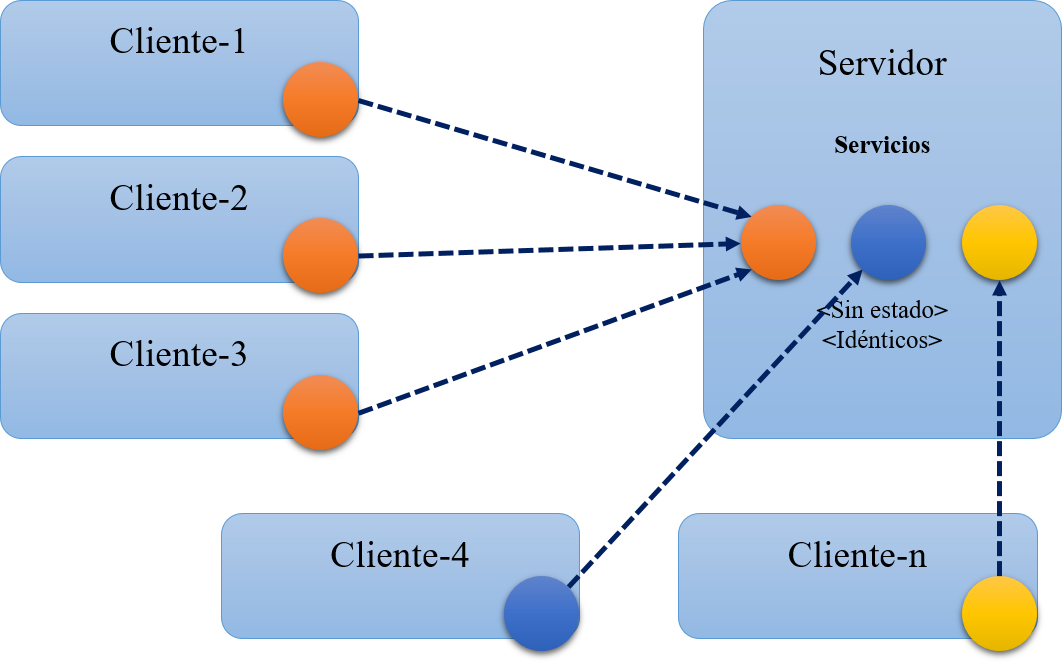
\includegraphics[width=10cm]{figures/ClienteServidorREST2.png} %NOMBRE DE LA FIGURA y TAMAÑO
        \caption{Servicios sin estado de la arquitectura cliente servidor REST} %PIE DE LA IMAGEN
        \label{arquitecturaREST2}
    \end{figure}
    
    \item Los servicios web tipo REST pueden guardar en cach\'e su contenido de tal manera que una vez realizada la primera petici\'on, el resto de peticiones puedan apoyarse en la cach\'e si fuera necesario,  ver la Figura \ref{arquitecturaREST3}.
    
    \begin{figure}[!ht]
        \centering
        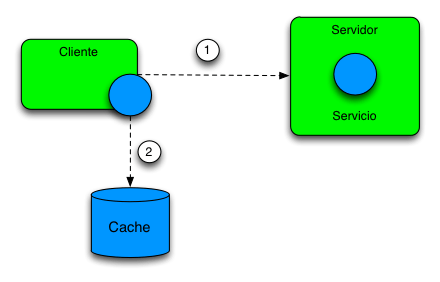
\includegraphics[width=10cm]{figures/ClienteServidorREST3.png} %NOMBRE DE LA FIGURA y TAMAÑO
        \caption{Servicios REST apoyados en cach\'e} %PIE DE LA IMAGEN
        \label{arquitecturaREST3}
    \end{figure}
    
    \item Todos lo servicios REST son \emph{uniformes}, es decir, comparten una forma de invocaci\'on y m\'etodos \url{GET, POST, PUT, DELETE}, ver la Figura \ref{arquitecturaREST4}.
    
    \begin{figure}[!ht]
        \centering
        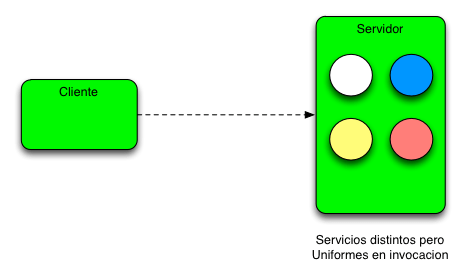
\includegraphics[width=10cm]{figures/ClienteServidorREST4.png} %NOMBRE DE LA FIGURA y TAMAÑO
        \caption{Servicios REST uniformes} %PIE DE LA IMAGEN
        \label{arquitecturaREST4}
    \end{figure}
    
    \item Los servicios REST son escalables y para el cliente transparentes, es decir, el cliente no puede distinguir si la petici\'on es atendida directamente por el servidor o por el sistema de cach\'es debido al servicio de balanceo de cargas, ver la Figura \ref{arquitecturaREST5}.
    
    \begin{figure}[!ht]
        \centering
        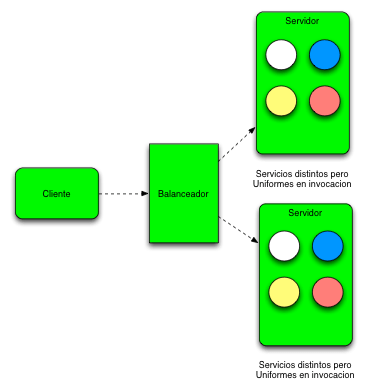
\includegraphics[width=10cm]{figures/ClienteServidorREST5.png} %NOMBRE DE LA FIGURA y TAMAÑO
        \caption{Arquitectura de capas de los servicios REST} %PIE DE LA IMAGEN
        \label{arquitecturaREST5}
    \end{figure}
    
\end{itemize}

Si bien algunos repositorios institucionales (RIs) cuentan con servicios tipo REST, el grado de complejidad en las consultas que hasta el momento est\'an implementadas, consideran s\'olo un atributo o caracter\'istica de los documentos, lo cual restringe el tipo de informaci\'on que puede recuperarse. El RN ofrece un cat\'alogo de m\'as de doscientos servicios REST \footnote{Disponible en: \textit{https://www.repositorionacionalcti.mx/docs/manualesInteroperabilidad}} que estan disponibles para aquellos usuarios que requieren informaci\'on (en formato JSON) \cite{CatalogoRESTRN} de cualquiera de los apartados mostrados en el cuadro \ref{descripcionserviciosRESTRN}.

\begin{table}[htbp]
\caption{Cat\'alogo de servicios REST ofrecidos por el RN} %Leyenda de la tabla
\begin{tabular}{| p{7cm}| p{7cm} |} \hline
\'areas de conocimiento          & Licencia                       \\ \hline
Campos de conocimiento         & Localidad                      \\ \hline
Disciplinas de conocimiento    & Municipio                      \\ \hline
Subdisciplinas de conocimiento & Nivel de acceso                \\ \hline
Audiencia                      & Pa\'is                           \\ \hline
Estado                         & Persona                        \\ \hline
Instituci\'on                    & Formato                        \\ \hline
Idioma                         & Programa                       \\ \hline
Financiador – Programa         & Proyecto                       \\ \hline
\end{tabular}

\label{descripcionserviciosRESTRN}
\end{table}

%El RN cuenta con un cat\'algo de m\'as de doscientos servicios REST que regresan los resultados en formato JSON \cite{CatalogoREST_RN}. La Tabla \ref{descripcionServiciosRESTRN} muestra la descripci\'on general.

%\begin{table}[!ht]
%    \centering
%    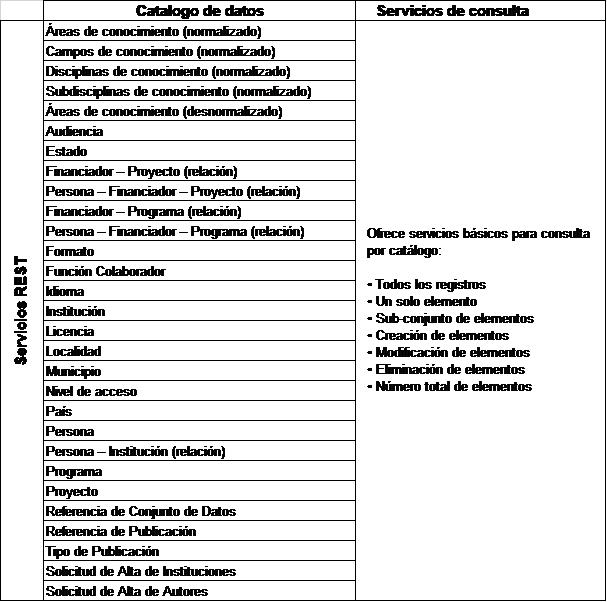
\includegraphics[width=10cm]{figures/TablaServiciosREST.png} %NOMBRE DE LA FIGURA y TAMAÑO
%    \caption{Descripci\'on de los servicios REST ofrecidos por el RN} %PIE DE LA IMAGEN
%    \label{descripcionServiciosRESTRN}
%\end{table}

Dependiendo del cat\'alogo, los servicios se consideran b\'asicos o espec\'ificos. La Figura \ref{ejemploConsumoRESTRN} muestra los elementos principales que intervienen en el consumo de un servicio del RN.\newline

\begin{figure}[!ht]
    \centering
    \fbox{
    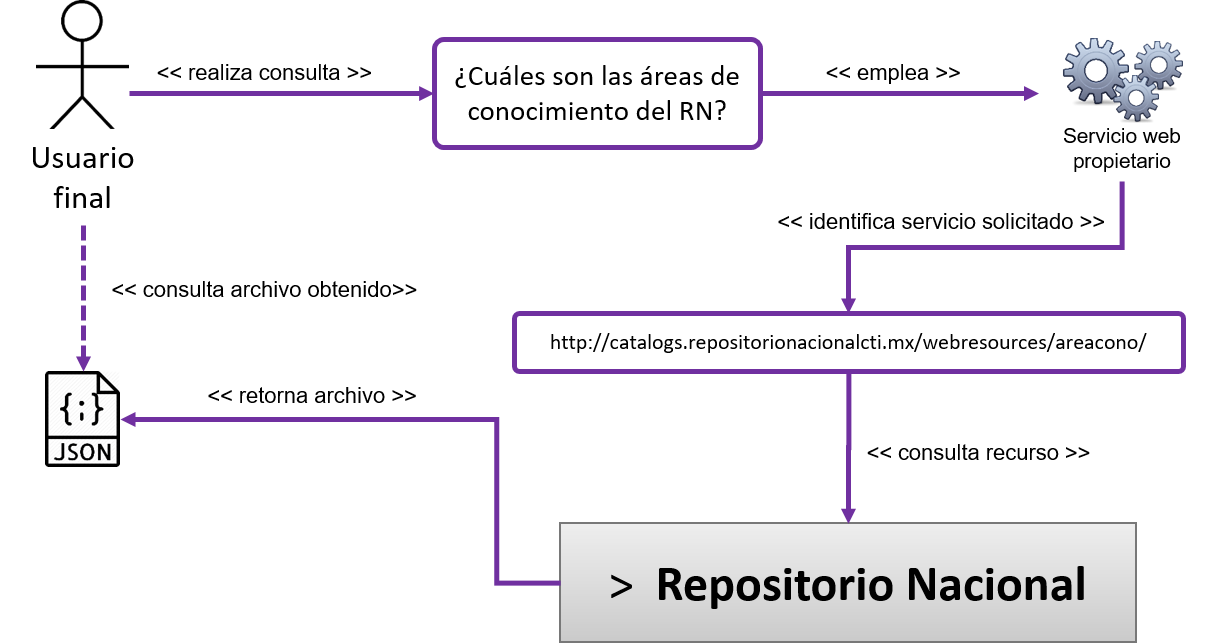
\includegraphics[scale=.75]{figures/ConsumoREST.png}} %NOMBRE DE LA FIGURA y TAMAÑO
    \caption{Ejemplo de consumo de un servicio REST del RN} %PIE DE LA IMAGEN
    \label{ejemploConsumoRESTRN}
\end{figure}

Los resultados de los servicios REST se almacenan en un archivo en formato \textit{JavaScript Object Notation} (JSON), formato de texto ligero utilizado para intercambiar datos. La Figura \ref{JSONejemploConsumoRESTRN} ilustra la manera en que un usuario o un agente consume un servicio REST.\newline

\begin{figure}[!ht]
    \centering
    \fbox{
    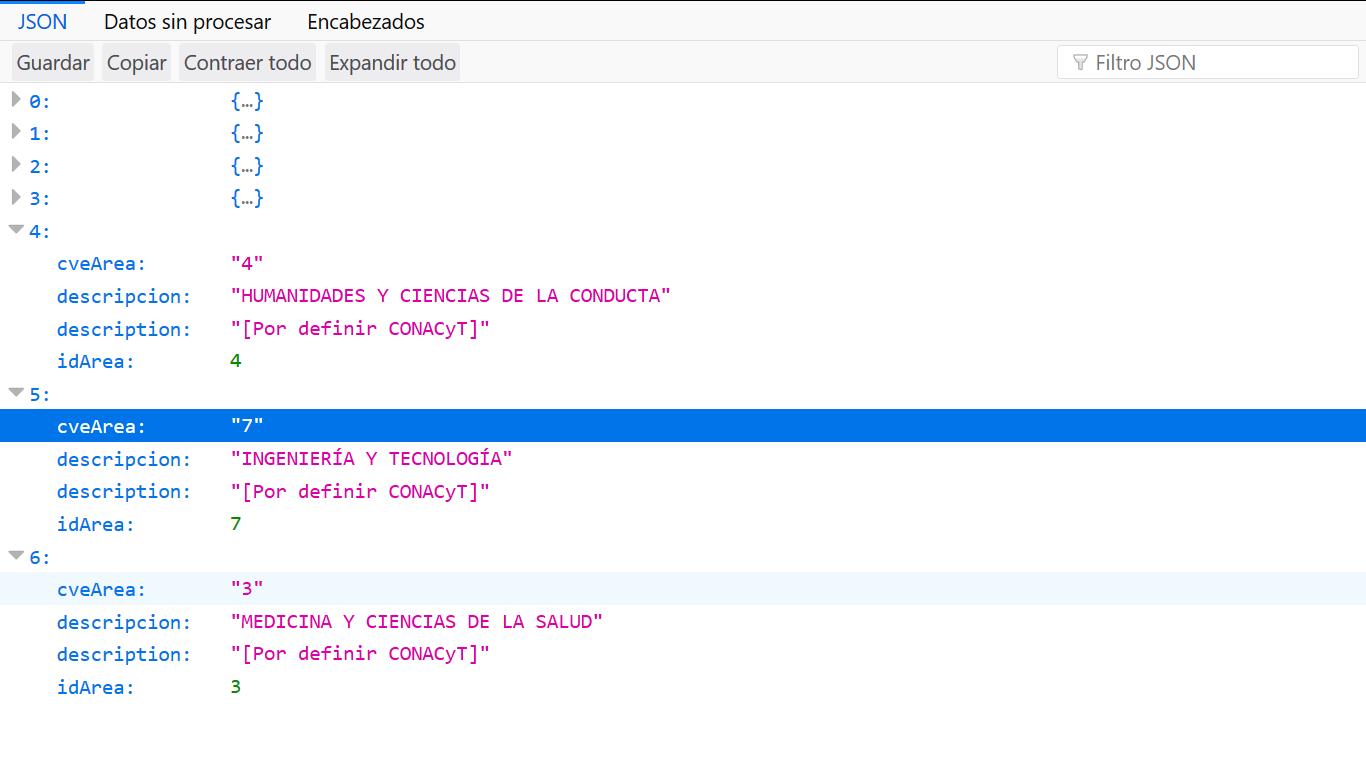
\includegraphics[scale=.45]{figures/JSONservicioRESTRN.png}} %NOMBRE DE LA FIGURA y TAMAÑO
    \caption{Archivo tipo JSON obtenido mediante servicio REST del RN} %PIE DE LA IMAGEN
    \label{JSONejemploConsumoRESTRN}
\end{figure}

El uso del protocolo REST permite el intercambio y manipulaci\'on de datos a trav\'es de Internet, lo cual contribuye al desarrollo de diversas aplicaciones y servicios web que usan datos con diversos or\'igenes. REST funge como interfaz entre un RI que use HTTP para obtener datos o generar operaciones sobre esos datos en formatos como XML y JSON. 

\section{COAR}

Uno de los aspectos que no aportan a la igualdad y libre acceso a la informaci\'on es la publicaci\'on en medios tradicionales, cuyos incentivos coorporativos ponen en desventaja a aquellos que no cuentan con acceso a sus plataformas, medios digitales o impresos. Para las IES y CI que distribuyen documentos en AA, diversos medios han apoyado la difusi\'on de la investigaci\'on y de la producci\'on acad\'emica que se caracterizan por recuperar documentos a partir de palabras clave. En 2016, la \emph{Confederation of Open Access Repositories},  Confederaci\'on de Repositorios de Acceso Abierto (COAR) integr\'o el equipo de trabajo \textit{Next Generation Repository Working Group}, equipo de trabajo para la siguiente generaci\'on de repositorios, cuyo prop\'osito fue definir las funcionalidades y tecnolog\'ias a desarrollar en los RDs en los pr\'oximos a\~{n}os. El informe \textit{Behaviours and Technical Recommendations of the COAR Next Generation Repositories} \cite{NextGenerationRepositories} es resultado de los trabajos, \'este indica que ser\'a necesario adoptar nuevas tecnolog\'ias, est\'andares y protocolos que permitan una mejor integraci\'on de los repositorios en los entornos web, de esta manera, los RDs jugar\'an un papel importante en el amplio campo de la comunicaci\'on acad\'emica. El informe plantea las siguientes caracter\'isticas para que los RDs sean fuentes s\'olidas de publicaci\'on, confiables y de AA \cite{NextGenerationRepositories}:

\begin{itemize}
\item Exponer \textit{identificadores}
\item Declaraci\'on de \textit{licencias} a nivel de recursos
\item Descubrimientos a trav\'es de la \textit{navegaci\'on}
\item Interactuar con \textit{recursos}
\item Descrubrimiento de \textit{lotes}
\item \textit{Transferencia} de recursos
\item \textit{Metadatos} de la actividad de recopilaci\'on y exposici\'on de la informaci\'on
\item \textit{Identificaci\'on} del usuario
\item \textit{Autenticaci\'on} del usuario
\item Exponer \textit{m\'etricas} de uso estandarizadas
\item \textit{Conservaci\'on} de los recursos
\end{itemize}

La visi\'on general del informe marca que, se deben establecer comunidades de investigadores y acad\'emicos que, por un lado, aporten al acervo de los repositorios, por otro lado, que al mismo tiempo incentiven la producci\'on en su comunidad o en otras comunidades interesadas en participar, de tal manera que los repositorios brinden una visi\'on global de la investigaci\'on cient\'ifica y acad\'emica. La tesis propone la implementaci\'on de un servicio web tipo REST conforme a la arquitectura que muestra la Figura \ref{arquitect1} como alternativa tecnol\'ogica acorde con algunos de los elementos del informe.

\begin{figure}[!ht]
    \centering
    \fbox{
    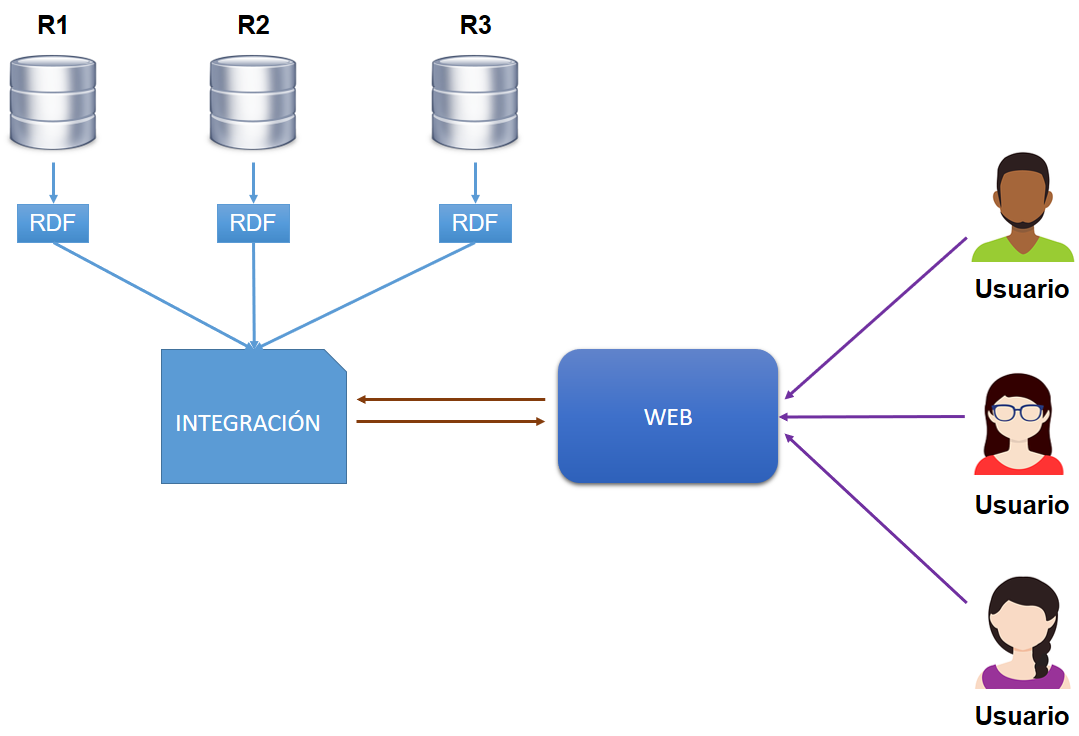
\includegraphics[width=10cm]{figures/ArquitecturaServicioWeb.png}} %NOMBRE DE LA FIGURA y TAMAÑO
    \caption{Arquitectura de servicio web sem\'antico} %PIE DE LA IMAGEN
    \label{arquitect1}
\end{figure}

\section{Trabajos relacionados}

La secci\'on de trabajos relacionados se integra de la revisi\'on documental y de sitios web que abordan tem\'aticas como repositorios, acceso abierto y tecnolog\'ias sem\'anticas. Por ejemplo, \cite{DrJulioSoler} plantea la transferencia de los resultados de investigaci\'on entre universidades o instituciones que, aunque los preservan, generan y transmiten, la transferencia se requiere sea lo m\'as eficiente y efectiva posible, produciendo resultados favorables para los involucrados. Al mismo tiempo, se se\~{n}ala la importancia de la representaci\'on de un dominio adecuado de la gesti\'on de la informaci\'on cient\'ifica definido mediante una ontolog\'ia sobre un software licenciado para la gesti\'on de contenidos (\emph{Content Management System}, sistema de administraci\'on de contenidos (CMS) y contenidos enriquecidos sem\'anticamente.\newline 

La Referencia, Red de Repositorios de Acceso Abierto a la Ciencia \cite{LaReferencia} \footnote{Disponible en: http://www.lareferencia.info/es/}, brinda un espacio para la divulgaci\'on de la ciencia en Latinoam\'erica, incluye en su cat\'alogo repositorios de pa\'ises como Argentina, Brasil, Chile, Colombia, Costa Rica, Ecuador, El Salvador, M\'exico y Per\'u. En los contenidos, los usuarios pueden consultar nodos nacionales, documentos varios, art\'iculos, reportes, tesis de maestr\'ia y doctorado. La Figura \ref{laReferencia} muestra estad\'isticas generales de LA-Referencia. 

\begin{figure}[!ht]
    \centering
    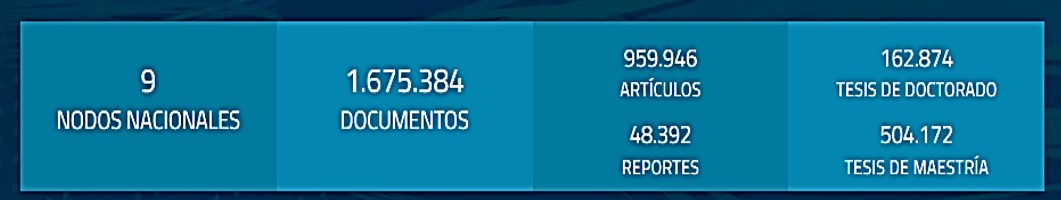
\includegraphics[width=14cm]{figures/lareferencia1.jpg} %NOMBRE DE LA FIGURA y TAMAÑO
    \caption{Estad\'isticas generales reportadas en LA Referencia} %PIE DE LA IMAGEN
    \label{laReferencia}
\end{figure}

OpenDOAR \footnote{Disponible en: http://v2.sherpa.ac.uk/opendoar/} es un directorio global de repositorios de acceso abierto acad\'emico. Permite la identificaci\'on, navegaci\'on y b\'usqueda en funci\'on de una serie de caracter\'isticas de los repositorios como la ubicaci\'on, el software o el tipo de material que se posee. \newline

Al mes de Octubre de 2019, OpenDOAR reporta las estad\'isticas de crecimiento por tipo de plataformas tecnol\'ogicas empleadas por los repositorios de acceso abierto (RAAs), ver Figura \ref{opendoarEstadisticas1}.

\begin{figure}[!ht]
    \centering
    \fbox{
    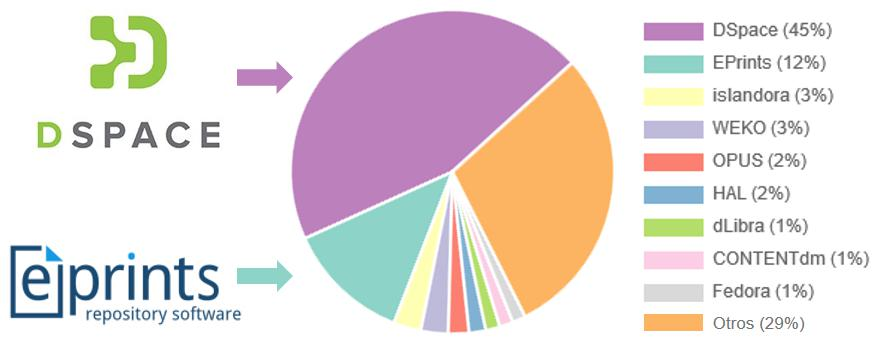
\includegraphics[width=12cm]{figures/opendoar3.jpg}} %NOMBRE DE LA FIGURA y TAMAÑO
    \caption{Repositorios por pa\'is en OpenDOAR} %PIE DE LA IMAGEN
    \label{opendoarEstadisticas1}
\end{figure}

\begin{figure}[!ht]
    \centering
    \fbox{
    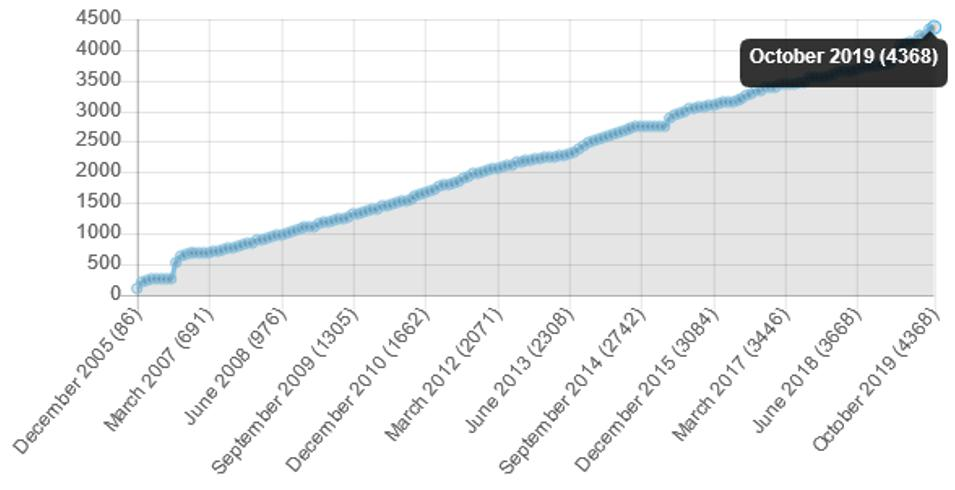
\includegraphics[width=12cm]{figures/opendoar4.jpg}} %NOMBRE DE LA FIGURA y TAMAÑO
    \caption{Repositorios por lenguaje y tipo de software en OpenDOAR} %PIE DE LA IMAGEN
    \label{opendoar_estadisticas_2}
\end{figure}

En Latinoam\'erica, LA Referencia reporta la producci\'on de recursos de AA que muestra la Tabla \ref{produccionRaas} y el tipo de servicios de b\'usqueda disponibles para los usuarios, notar que los atributos recurrentes para las b\'usquedas b\'asicas son: t\'itulo y autor, mientras que en el caso de las avanzadas, el n\'umero de par\'ametros de b\'usqueda var\'ia entre cuatro y doce. Finalmente, se pudo identificar que, ninguno de los repositorios consultados cuenta con  servicio de b\'usqueda sem\'antica.

%\begin{figure}[!ht]
%    \centering
%    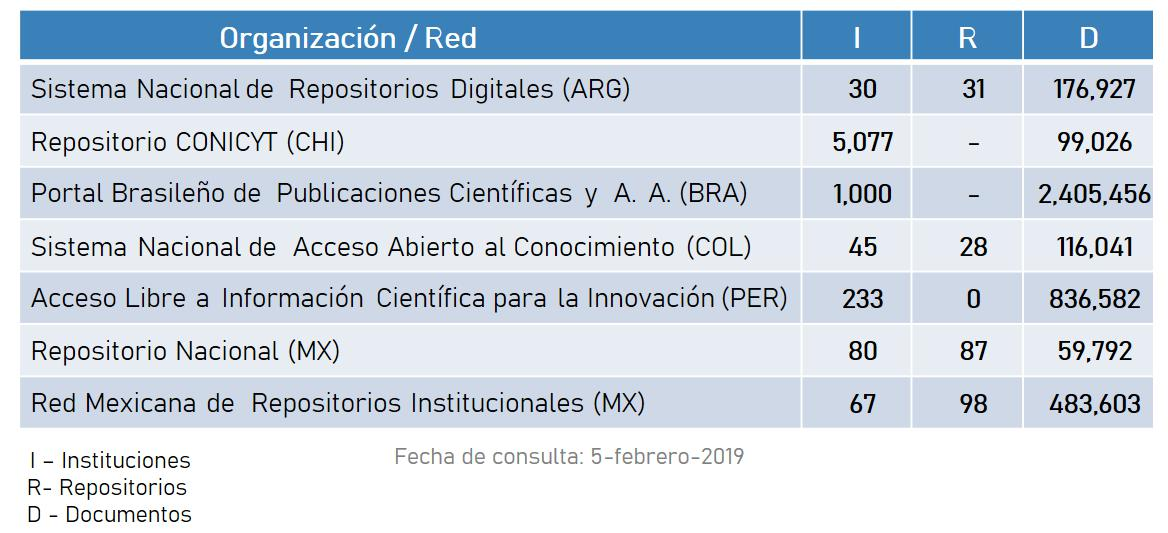
\includegraphics[width=14cm]{figures/estadisticasRaas.jpg}
%    \caption{Repositorios con mayor producci\'on en Latinoam\'erica} %PIE DE LA IMAGEN
%    \label{estadisticasRaas}
%\end{figure}

\begin{table}[htbp]
\caption{Repositorios con mayor producci\'on en Latinoam\'erica}
\begin{tabular}{| p{9.5cm}| p{1.5cm} | p{1.5cm} | p{1.5cm} |}
\hline
\multicolumn{1}{|c|}{\textbf{Organizaci\'on / Red}}                                    & \multicolumn{1}{c|}{\textbf{I}}     & \multicolumn{1}{c|}{\textbf{R}}  & \multicolumn{1}{c|}{\textbf{D}}         \\ \hline
\multicolumn{1}{|l|}{Sistema Nacional de  Repositorios Digitales (ARG)}              & \multicolumn{1}{c|}{\textbf{30}}    & \multicolumn{1}{c|}{\textbf{31}} & \multicolumn{1}{c|}{\textbf{176,927}}   \\ \hline
\multicolumn{1}{|l|}{Repositorio CONICYT (CHI)}                                      & \multicolumn{1}{c|}{\textbf{5,077}} & \multicolumn{1}{c|}{\textbf{-}}  & \multicolumn{1}{c|}{\textbf{99,026}}    \\ \hline
\multicolumn{1}{|l|}{Portal Brasileño de  Publicaciones Cient\'ificas y  A. A. (BRA)}  & \multicolumn{1}{c|}{\textbf{1,000}} & \multicolumn{1}{c|}{\textbf{-}}  & \multicolumn{1}{c|}{\textbf{2,405,456}} \\ \hline
\multicolumn{1}{|l|}{Sistema Nacional de  Acceso Abierto al Conocimiento (COL)}      & \multicolumn{1}{c|}{\textbf{45}}    & \multicolumn{1}{c|}{\textbf{28}} & \multicolumn{1}{c|}{\textbf{116,041}}   \\ \hline
\multicolumn{1}{|l|}{Acceso Libre a Informaci\'on Cient\'ifica para la Innovaci\'on (PER)} & \multicolumn{1}{c|}{\textbf{233}}   & \multicolumn{1}{c|}{\textbf{0}}  & \multicolumn{1}{c|}{\textbf{836,582}}   \\ \hline
\multicolumn{1}{|l|}{Repositorio Nacional (MX)}                                      & \multicolumn{1}{c|}{\textbf{80}}    & \multicolumn{1}{c|}{\textbf{87}} & \multicolumn{1}{c|}{\textbf{59,792}}    \\ \hline
\multicolumn{1}{|l|}{Red Mexicana de  Repositorios Institucionales (MX)}             & \multicolumn{1}{c|}{\textbf{67}}    & \multicolumn{1}{c|}{\textbf{98}} & \multicolumn{1}{c|}{\textbf{483,603}}  \\ \hline
\end{tabular}
\label{produccionRaas}
\footnotesize{ \textbf{\textit{I - Instituciones, R - Repositorios, D - Documentos}}}
\end{table}

%\begin{figure}[!ht]
%    \centering
%    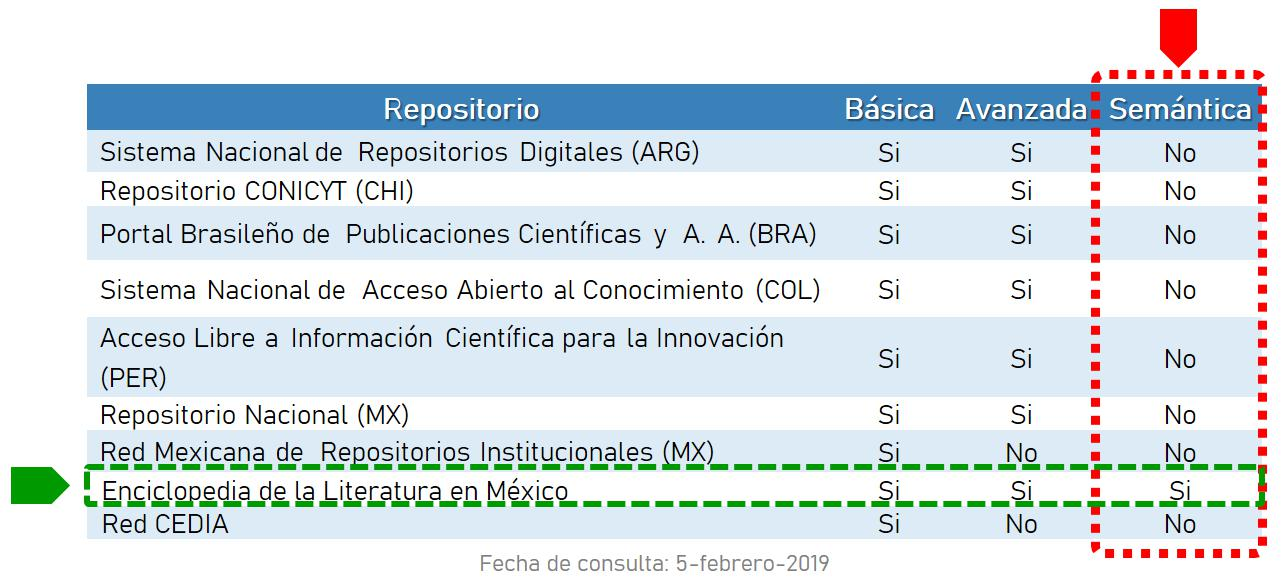
\includegraphics[width=14cm]{figures/serviciosBusquedaSemantica1.jpg} %NOMBRE DE LA FIGURA y TAMAÑO
%    \caption{Servicios de b\'usqueda en RAAs} %PIE DE LA IMAGEN
%    \label{busquedas-raas}
%\end{figure}

\begin{table}[htbp]
\caption{Servicios de b\'usquedas en RAAs}
\begin{tabular}{| p{8.5cm}| p{1.5cm} | p{2cm} | p{2cm} |}
\hline
\multicolumn{1}{|c|}{\textbf{Repositorio}}                     & \textbf{B\'asica} & \textbf{Avanzada} & \textbf{Sem\'antica} \\ \hline
Sistema Nacional de  Repositorios Digitales (ARG)              & Si              & Si                & No                 \\ \hline
Repositorio CONICYT (CHI)                                      & Si              & Si                & No                 \\ \hline
Portal Brasileño de  Publicaciones Cient\'ificas y  A. A. (BRA)  & Si              & Si                & No                 \\ \hline
Sistema Nacional de  Acceso Abierto al Conocimiento (COL)      & Si              & Si                & No                 \\ \hline
Acceso Libre a Informaci\'on Cient\'ifica para la Innovaci\'on (PER) & Si              & Si                & No                 \\ \hline
Repositorio Nacional (MX)                                      & Si              & Si                & No                 \\ \hline
Red Mexicana de  Repositorios Institucionales (MX)             & Si              & No                & No                 \\ \hline
Enciclopedia de la Literatura en M\'exico                        & Si              & Si                & Si                 \\ \hline
Red CEDIA                                                      & Si              & No                & No                 \\ \hline
\end{tabular}
\label{busquedasRaas}
\end{table}

Las figuras \ref{snrd1} a  \ref{alicia-1} muestran las p\'aginas iniciales de los repositorios consultados y secciones de la interfaz correspondientes a sus m\'odulos de b\'usqueda.

\begin{figure}[!ht]
    \centering
    \fbox{
    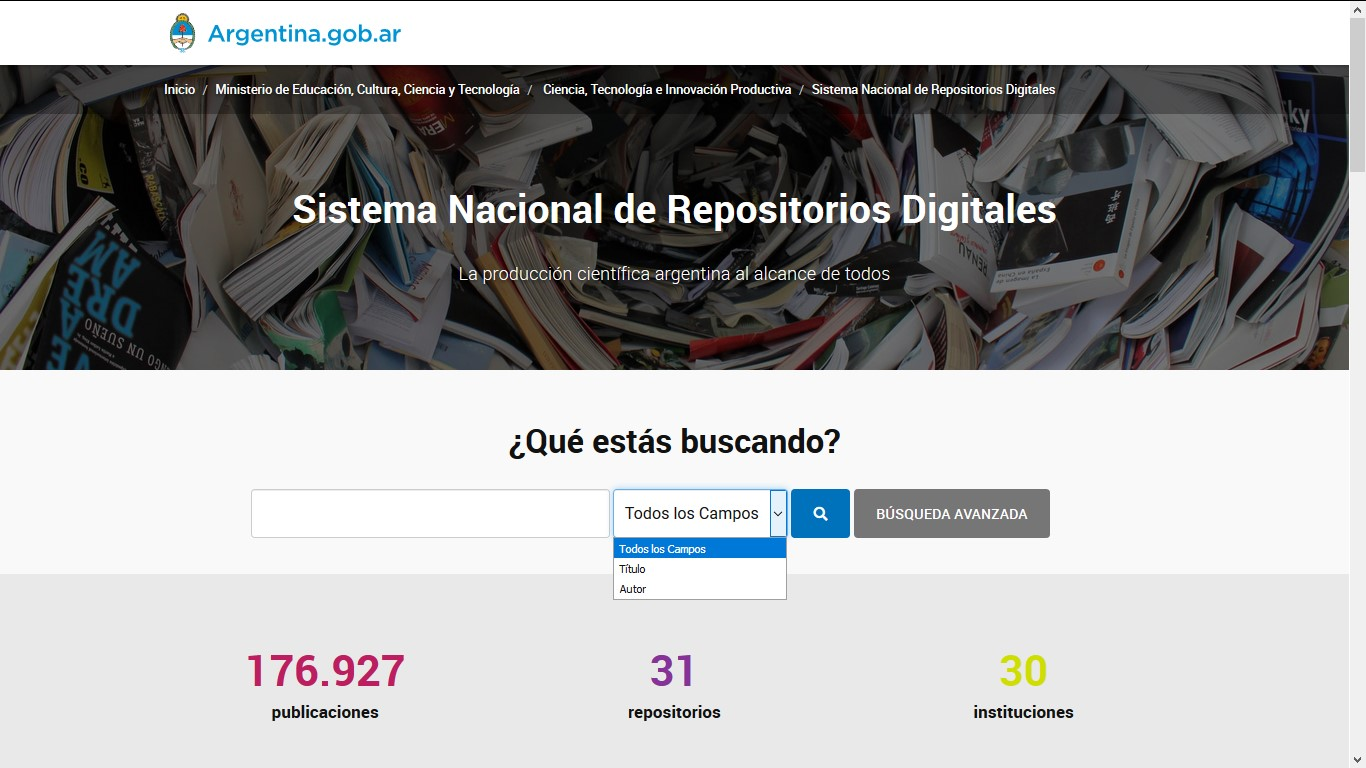
\includegraphics[width=14cm]{figures/repositoriosnrdarg1.jpg}}
    \caption{Vista del portal del Sistema Nacional de Repositorios Digitales} %PIE DE LA IMAGEN
    \label{snrd1}
\end{figure}

\begin{figure}[!ht]
    \centering
    \fbox{
    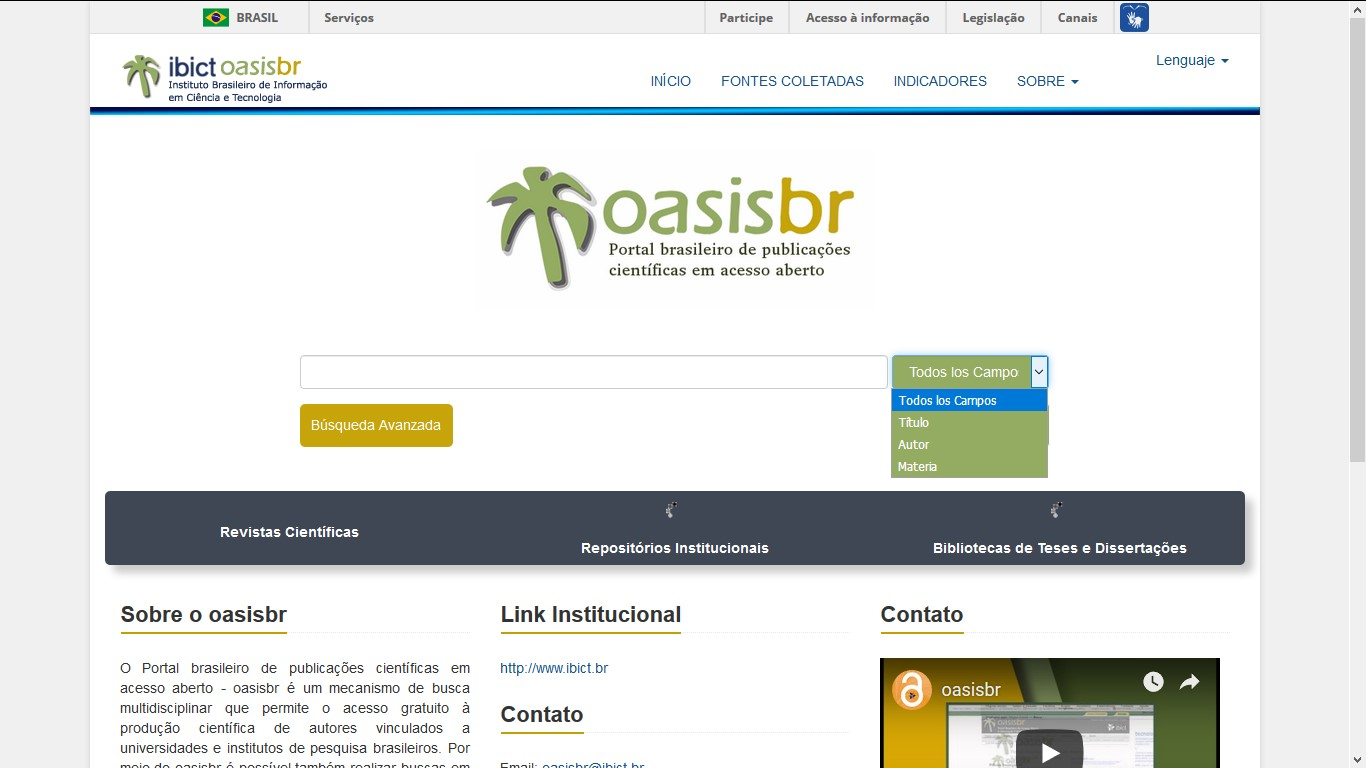
\includegraphics[width=14cm]{figures/repositoriosnrdbr1.jpg}} %NOMBRE DE LA FIGURA y TAMAÑO
    \caption{Vista del portal brasile\~{n}o de publicaciones cient\'ificas y acceso abierto - oasisbr} %PIE DE LA IMAGEN
    \label{oasisbr-1}
\end{figure}

\begin{figure}[!ht]
    \centering
    \fbox{
    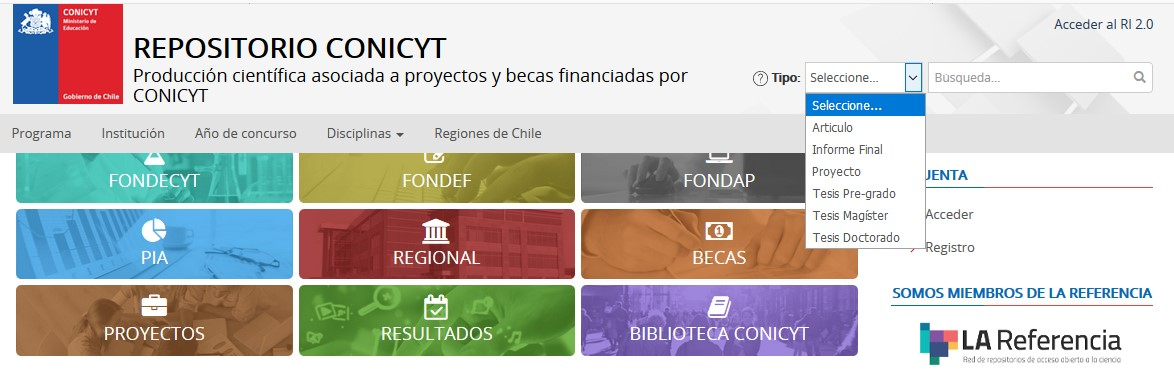
\includegraphics[width=14cm]{figures/repositorioconicytchi3.jpg}} %NOMBRE DE LA FIGURA y TAMAÑO
    \caption{Vista del panel de b\'usquedas en RI2.0} %PIE DE LA IMAGEN
    \label{ri2.0-2}
\end{figure}

\begin{figure}[!ht]
    \centering
    \fbox{
    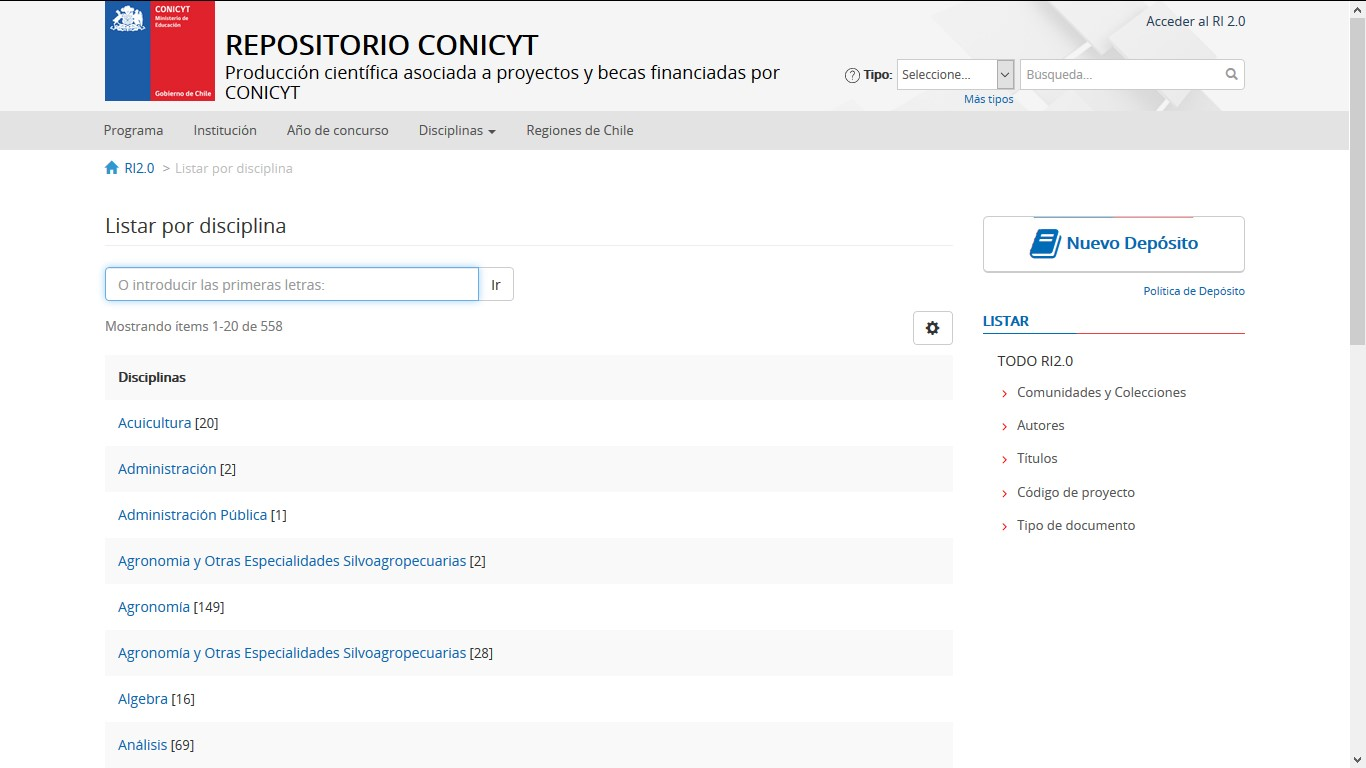
\includegraphics[width=14cm]{figures/repositorioconicytchi2.jpg}} %NOMBRE DE LA FIGURA y TAMAÑO
    \caption{Vista del panel de b\'usquedas avanzadas en RI2.0} %PIE DE LA IMAGEN
    \label{ri2.0-3}
\end{figure}

\begin{figure}[!ht]
    \centering
    \fbox{
    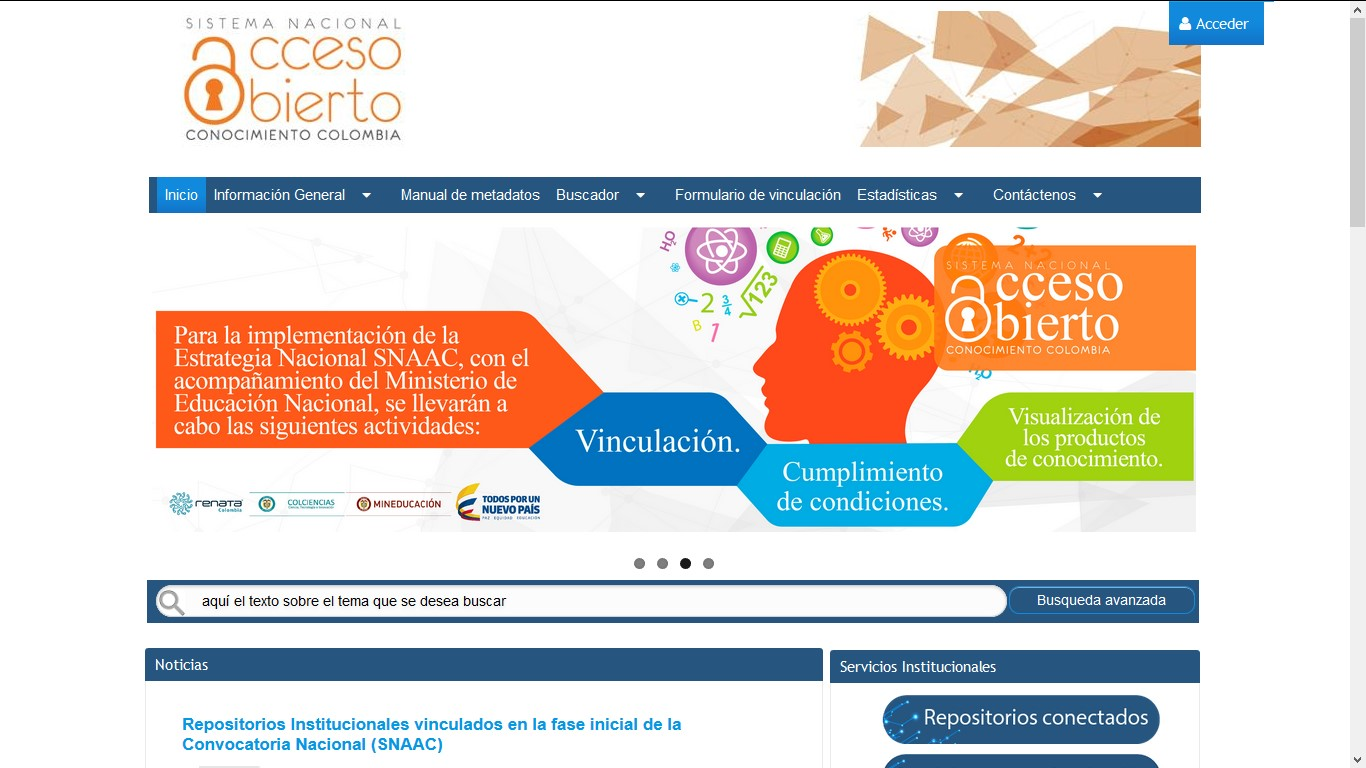
\includegraphics[width=14cm]{figures/repositoriosnaac1.jpg}} %NOMBRE DE LA FIGURA y TAMAÑO
    \caption{Vista del Sistema Nacional de Acceso Abierto al Conocimiento} %PIE DE LA IMAGEN
    \label{snaac-1}
\end{figure}

\begin{figure}[!ht]
    \centering
    \fbox{
    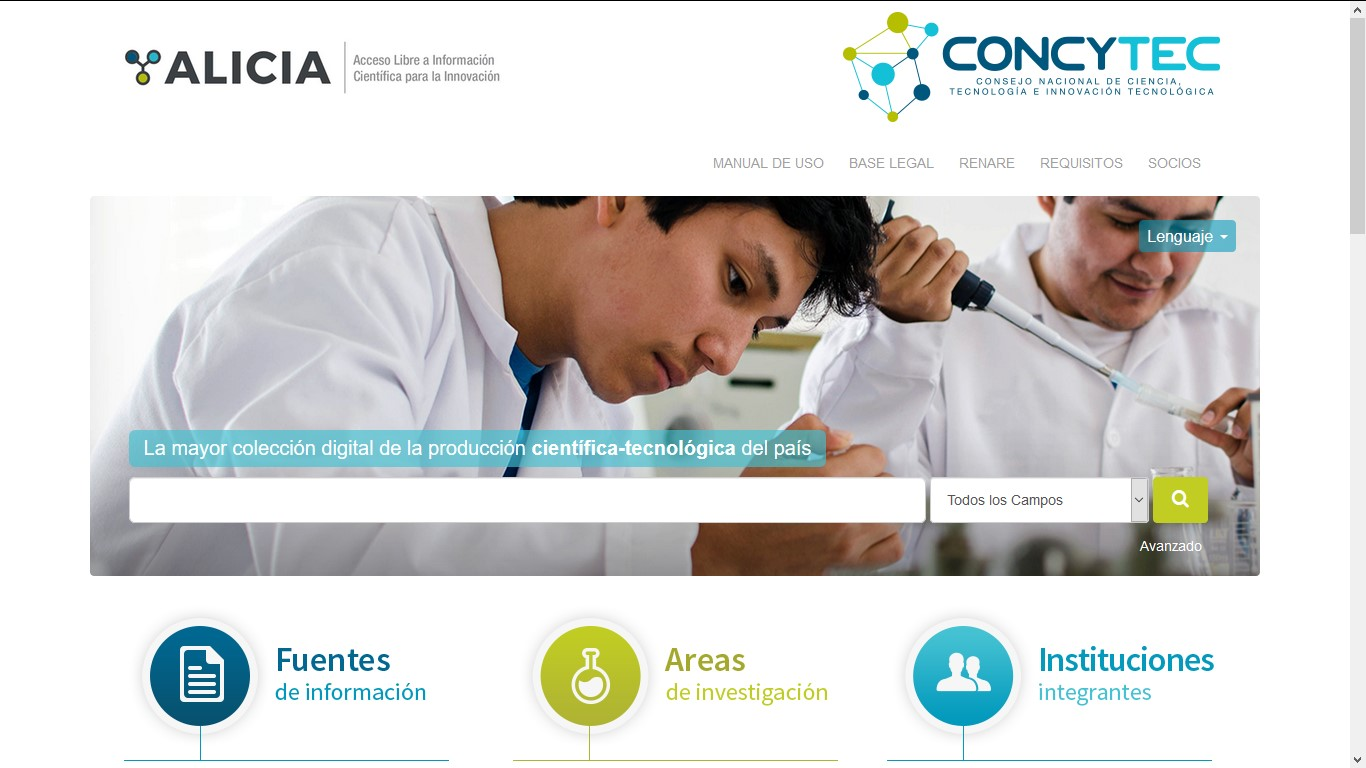
\includegraphics[width=14cm]{figures/repositorioaliciaperu1.jpg}} %NOMBRE DE LA FIGURA y TAMAÑO
    \caption{Vista del portal de acceso libre a informaci\'on cient\'ifica para la innovaci\'on} %PIE DE LA IMAGEN
    \label{alicia-1}
\end{figure}

\subsection{Servicios de b\'usqueda simple, avanzada y sem\'antica}

Las figuras \ref{busquedas-snrd-1} y \ref{busquedas-snrd-2} muestran los servicios de b\'usqueda que ofrecen diferentes RAAs a sus usuarios, basados en criterios de filtrado que en general son comunes tales como el autor, t\'itulo, editor, lenguaje, fecha de publicaci\'on, entre otros.\newline

\begin{figure}[!ht]
    \centering
    \fbox{
    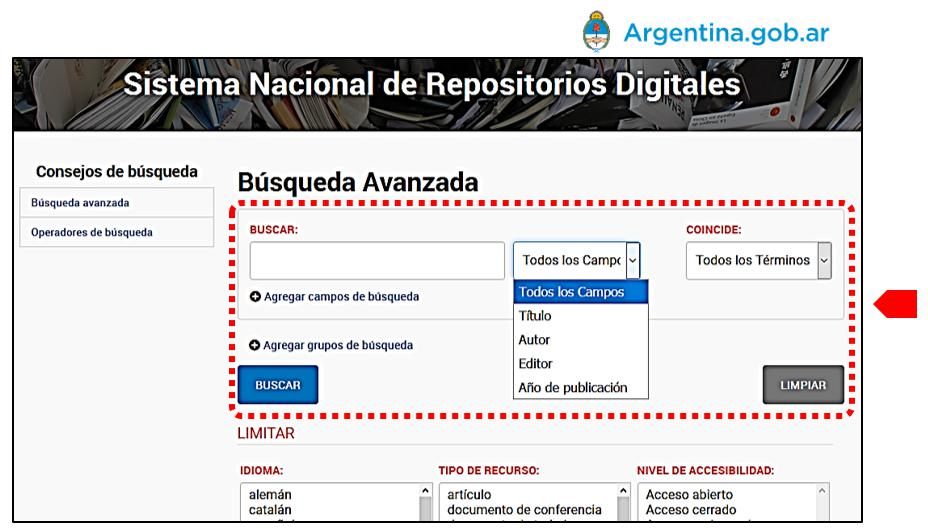
\includegraphics[width=14cm]{figures/BusquedasARG.jpg}} %NOMBRE DE LA FIGURA y TAMAÑO
    \caption{Vista del panel de b\'usqueda en el portal Sistema Nacional de Repositorios Digitales en Argentina} %PIE DE LA IMAGEN
    \label{busquedas-snrd-1}
\end{figure}

\begin{figure}[!ht]
    \centering
    \fbox{
    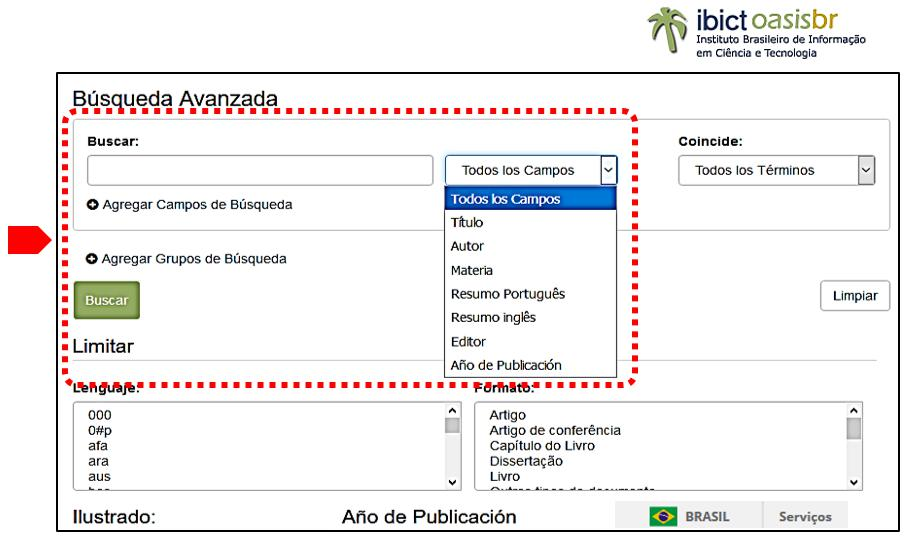
\includegraphics[width=14cm]{figures/BusquedasBRA.jpg}} %NOMBRE DE LA FIGURA y TAMAÑO
    \caption{Vista del panel de b\'usqueda en el portal instituto Brasile\~{n}o de Informaci\'on en Ciencia y Tecnolog\'ia en Brasil} %PIE DE LA IMAGEN
    \label{busquedas-snrd-2}
\end{figure}

La figura \ref{busquedasRaas} concentra informaci\'on de los portales con mayor producci\'on en Latinoam\'erica y los servicios de b\'usqueda que ofrecen, notar que s\'solo uno de los repositorios ofrece servicios basados en tecnolog\'ias sem\'anticas.
\subsection{Comparativa entre plataformas}

Los RAAs cuentan con diversas caracter\'isticas t\'ecnicas que permiten implementar servicios para sus usuarios. Para la implementaci\'on de servicios sem\'anticos se requiere observar tres caracter\'isticas:

\begin{itemize}
    \item Servicio o m\'odulo RDF
    \item Proveedor de almacenamiento de ternas
    \item Lenguaje de consulta
\end{itemize}{}

La tabla \ref{tabla_comparativa} muestra las caracter\'isticas t\'ecnicas entre las plataformas DSpace, Virtuoso y VIVO.\newline

\begin{table}[htbp]
    \begin{center}
    \caption{Tabla comparativa de caracter\'isticas t\'ecnicas entre plataformas DSpace, Virtuoso y VIVO}
    \begin{tabular}{| p{4cm}| p{3cm} |p{4cm} | p{3cm} |}
    \hline
    \centering \textbf{Plataforma} & \textbf{Servicio RDF} & \textbf{Proveedor de almacenamiento} & \textbf{Lenguaje de consulta} \\
    \hline \hline
    DSpace 6.2 & Si & Apache Jena & SPARQL \\ \hline
    Virtuoso & Si & Sesame, Redland, Apache Jena & SPARQL \\ \hline
    VIVO & Si & - & SPARQL \\ \hline
    \end{tabular}
    \label{tabla_comparativa}
    \end{center}
\end{table}

La Figura \ref{ejemploRDFternas} muestra el esquema RDF expresado como un conjunto de ternas, (tambi\'en llamadas tripletas).\newline

\begin{figure}[!ht]
    \centering
    \fbox{
    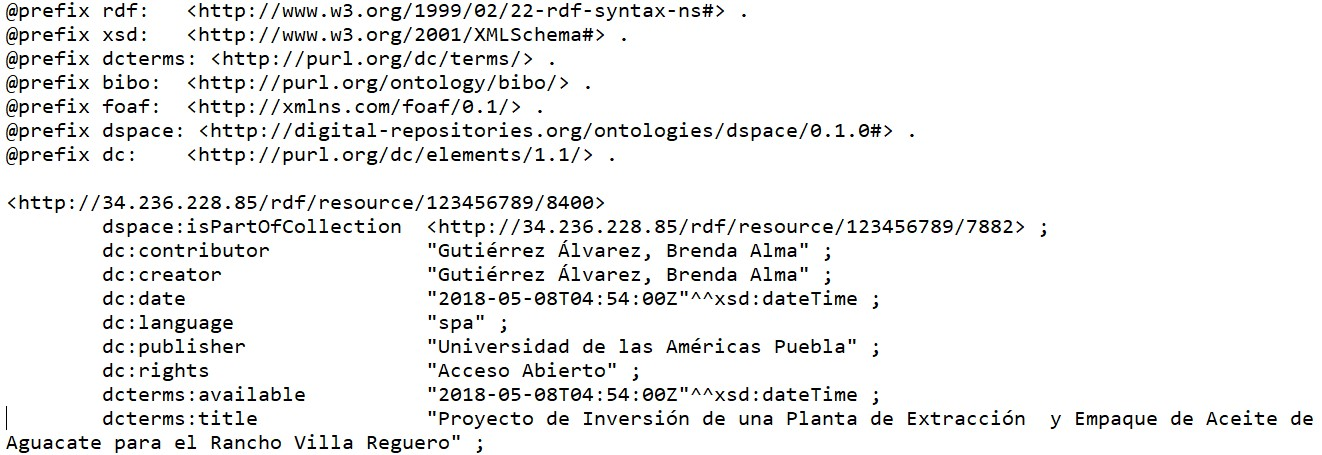
\includegraphics[width=14cm]{figures/ejemploRDF.jpg}} %NOMBRE DE LA FIGURA y TAMAÑO
    \caption{Ejemplo de conjunto de ternas en RDF} %PIE DE LA IMAGEN
    \label{ejemploRDFternas}
\end{figure}
  